%%%%%%%%%%%%%%%%%%%%%%%%%%%%%%%%%%%%%%%%%%%%%%%%%%%%%%%%%%%%
\newpage
\appendix


\section*{Appendix / supplemental material}
In the appendix, we provide additional experimental details~(Appendix~\ref{sec:experimental}), implementation details~(Appendix~\ref{sec:implementation}), qualitative results~(Appendix~\ref{sec:qualitative}), grounding consistency evaluation~(Appendix~\ref{sec:consistency}), more ablation studies~(Appendix~\ref{sec:ablation}), discussions of limitations and future work~(Appendix~\ref{sec:limitations}), and broader impacts~(Appendix~\ref{sec:impacts}).

%%%%%%%%%%%%%%%%%%%%%%%%%%%%%%%%%%%%%%%%%%%%%%%%%%%%%%%%%%%%
\section{Experimental Details}
\label{sec:experimental}

In this section, we provide additional experimental details, including benchmark details~(Appendix~\ref{sub:benchmarks}), ablation details~(Appendix~\ref{sub:ablation}), robustness test details~(Appendix~\ref{sub:robustness})and downsteam task details~(Appendix~\ref{sub:donwstream}).

\subsection{Benchmark Details}
\label{sub:benchmarks}
% \subsubsection{Benchmarks}
% \label{subsub:benchmarks}
% The statistics of evaluation benchmarks we used are listed in Table~\ref{table:benchmarks}. 
% The information about major benchmarks is introduced below.

% \paragraph{Short-video Temporal Grounding Benchmarks.} \textbf{Charades-STA}~\cite{sigurdsson2016hollywood} is an action recognition dataset that was later annotated for video grounding. The videos are approximately 31 seconds long, with an average event length of 8.1 seconds. The dataset is originally split into two subsets: training (12,408 samples) and test (3,720 samples).  
% \textbf{ANet-Captions}~\cite{krishna2017dense} was initially built for dense video captioning and later adapted for video grounding tasks. The videos have an average duration of two minutes, with events averaging 36 seconds in length. The dataset is divided into three splits: train (37,421 samples), val\_1 (17,505 samples), and val\_2 (17,031 samples).  
% \textbf{QVHighlights}~\cite{lei2021detecting} is one of the most recent benchmarks, containing 10,148 videos with an average duration of 150 seconds. These videos were cropped from YouTube content, and each is annotated with at least one query. The target temporal windows have an average length of 24.6 seconds. The dataset is split into training, validation, and test sets containing 7,218, 1,150, and 1,542 queries, respectively. We evaluate on the test set of Charades-STA, the val\_2 set of ANet-Captions, and the test set of QVHighlights (measured through submitting the prediction to the evaluation server\footnote{Evaluation server, QVHighlights: \href{https://codalab.lisn.upsaclay.fr/competitions/6937}{https://codalab.lisn.upsaclay.fr/competitions/6937}}).
% It is worth noting that the results of QVHighlights in Table~\ref{table:sota_table_zs} are evaluated on the validation set.
% In short-video temporal grounding benchmarks, the videos are generally shorter in duration, with events occupying a relatively larger proportion of the video. Consequently, temporal grounding in these benchmarks is relatively less challenging.

% \begin{table}[h]
% \caption{Statistics of benchmarks. The benchmarks encompass three representative tasks – Video Temporal Grounding, Grounded VideoQA, and General VideoQA. The reported statistics are based on the actual numbers of videos and queries used in our experiments.}
% \vspace{5pt}
% \centering
% \resizebox{\textwidth}{!}{
% % \setlength{\tabcolsep}{0.25cm}
% \begin{tabular}{l r r r r r r}
% \toprule
%  \textbf{Benchmark} & \textbf{\makecell[c]{\#Videos}} & \textbf{\makecell[c]{\#Queries}} & \textbf{\makecell[c]{Video Len.}} & \textbf{\makecell[c]{Moment Len.}} & \textbf{Views} & \textbf{Domain}\\
%  \midrule
%  Ego4D-NLQ~\cite{grauman2022ego4d} & 415 & 4.6K & 500s & 10.7s & Ego & Open \\
%  TACoS~\cite{regneri2013grounding} & 25 & 4.0K & 368s & 31.9s & Ego \& Exo & Cooking \\
%  Charades-STA~\cite{sigurdsson2016hollywood} & 1.3K & 3.7K & 29s & 7.8s & Exo & Activity \\
%  QVHighlights~\cite{lei2021detecting} & 1.5K & 1.5K & 150s & 32
%  .2s & Ego \& Exo & Vlog/News \\
%  ANet-Captions~\cite{krishna2017dense} & 4.9K & 17.0K & 118s & 40.2s & Ego \& Exo & Activity \\
%  QaEgo4D~\cite{barmann2022did} & 148 & 500 & 487s & 13s & Ego & Open \\
%  CG-Bench~\cite{cgbench} & 1.2K & 12K & 1661.1s & 19.8s & Ego \& Exo  & Open \\
%  MLVU~\cite{mlvu} & 1.1K & 2.2K & 755.7s & - & Ego \& Exo & Open \\
%  LongVideoBench~\cite{longvideobench} & 618 & 1.2K & 574.9s & - & Ego \& Exo & Open \\
%  \bottomrule
% \end{tabular}}
% \label{table:benchmarks}
% \end{table}

% \paragraph{Long-video Temporal Grounding Benchmarks.} \textbf{Ego4D-NLQ}~\cite{grauman2022ego4d} is a large-scale collection of egocentric videos capturing daily human activities. The second version of this benchmark, $NLQ_{v2}$, contains 1,659 video clips paired with 17.3K natural language queries and their corresponding temporal windows. The videos have an average duration of 495 seconds, while events last an average of 8.2 seconds. We evaluate on the validation set, which includes 415 videos with 4,552 queries.  
% \textbf{TACoS}~\cite{regneri2013grounding} is a traditional benchmark comprising 10.1 hours of cooking videos, with an average of 143.5 queries per video. The videos have an average duration of 287 seconds, and events last an average of 27.9 seconds. We evaluate on the test set, which includes 25 videos with 4,001 queries.
% In contrast to short-video benchmarks, long-video temporal grounding benchmarks involve significantly longer videos, with events occupying a much smaller proportion of the video. This creates considerable challenges for achieving precise temporal grounding.

% \paragraph{Grounded Video Question-answering Benchmarks.} Since the video duration in the current long-video temporal grounding Benchmarks is still relatively short, we evaluate our model's long video grounding capabilities on extremely long VideoQA Benchmarks with grounded temporal windows.  
% \textbf{QaEgo4D}~\cite{barmann2022did} is the multiple-choice subset of the QAEGO4D-test benchmark, focusing on question-answering in long egocentric videos. It includes annotations marking video segments relevant to each question. We evaluate on the test set, containing 148 videos with 500 queries.  
% \textbf{CG-Bench}~\cite{cgbench} is designed for long video grounded question-answering, featuring a diverse domain and various evaluation metrics. It includes 1.2K manually curated videos, ranging from 10 to 80 minutes, with a total of 12K QA pairs. The dataset is categorized into perception, reasoning, and hallucination question types, and introduces clue-based evaluation methods like white box and black box assessments to ensure models provide answers based on accurate video reasoning.  
% These grounded video question-answering Benchmarks not only assess the model's long-video temporal grounding capabilities but also explore how temporal grounding models contribute to video understanding.

% \paragraph{General Video Question-answering Benchmarks.} Due to the limited availability of video QA benchmarks with temporal window annotations, we explore the generalizability of our model on general long VideoQA benchmarks.  
% \textbf{MLVU}~\cite{mlvu} is designed to evaluate the long-form video understanding capabilities of multimodal large language models (MLLMs). The question-answer pairs are manually labeled and categorized into three groups: single-detail, multi-detail, and holistic. We evaluate on the multiple-choice subset.  
% \textbf{LongVideoBench}~\cite{longvideobench} is a benchmark that focuses on referring reasoning questions, where questions contain referring queries that require understanding specific video contexts (i.e., referred context) to provide accurate answers. We evaluate on the validation set.

% \subsubsection{Evaluation Metrics}
% \label{subsub:metrics}

To evaluate the performance of our model on temporal grounding and VideoQA tasks, we employ three key metrics: Intersection-over-Union (IoU), Intersection-over-Prediction (IoP), and Intersection-over-Ground Truth (IoG). These metrics quantify the alignment between the predicted temporal window \( T^{\text{pred}} \) and the ground truth temporal window \( T^{\text{gt}} \). The formal definitions are as follows:
\begin{equation*}
    \text{IoU} = \frac{|T^{\text{pred}} \cap T^{\text{gt}}|}{|T^{\text{pred}} \cup T^{\text{gt}}|}, \quad
    \text{IoP} = \frac{|T^{\text{pred}} \cap T^{\text{gt}}|}{|T^{\text{pred}}|}, \quad
    \text{IoG} = \frac{|T^{\text{pred}} \cap T^{\text{gt}}|}{|T^{\text{gt}}|}.
\end{equation*}

Here, \( |T^{\text{pred}} \cap T^{\text{gt}}| \) denotes the duration of the overlapping region between the predicted window \( T^{\text{pred}} \) and the ground truth window \( T^{\text{gt}} \). \( |T^{\text{pred}} \cup T^{\text{gt}}| \) represents the duration of their union, while \( |T^{\text{pred}}| \) and \( |T^{\text{gt}}| \) denote the durations of the predicted and ground truth windows, respectively.

IoU measures the overall alignment between \( T^{\text{pred}} \) and \( T^{\text{gt}} \), providing a balanced assessment of both precision and recall by considering the overlap relative to their union. IoP emphasizes precision, indicating the proportion of the predicted window that overlaps with the ground truth. Conversely, IoG focuses on recall, reflecting the proportion of the ground truth window that is covered by the prediction. Collectively, these metrics offer a comprehensive evaluation of the model's ability to accurately localize temporal windows with respect to the ground truth.

\subsection{Ablation Details}
\label{sub:ablation}
\subsubsection{Effect of Individual Modules}
\label{subsub:individual}

As shown in Table~\ref{table:abl_cumu}, we systematically evaluate the effect of each individual module. The detailed settings are as follows:
(i) \textbf{Row 1}: We uniformly sample 32 frames from each video and obtain the corresponding timestamps. These frames and timestamps are then fed into UniTime for temporal grounding.
(ii) \textbf{Row 2}: We sample the video at 2 fps and apply frame scaling. The sampled frames and their timestamps are input into UniTime for temporal grounding.
(iii) \textbf{Row 3}: On top of uniform sampling, we introduce multi-stage inference. Specifically, after obtaining an initial prediction using the uniformly sampled frames (as in row 1), we perform a second round of uniform sampling within the predicted interval and feed these frames into the model for refined localization.
(iv) \textbf{Row 4}: Similarly, we apply multi-stage inference to the adaptive frame scaling. After the initial prediction (as in row 2), we resample at 2 fps and apply frame scaling within the predicted interval, then input these frames into the model for further refinement.
(v) \textbf{Row 5}: We adopt the coarse-to-fine temporal grounding strategy described in Section~\ref{sec:architecture}. Unlike row 4, where the model predicts fine-grained intervals in the first round due to densely sampled timestamps, row 5 partitions the video into coarse segments and only requires the model to predict the relevant segment in the first round. In the second round, temporal grounding is performed within the selected segment to localize the precise moment.

\subsubsection{Effect of Segment Length and Replication Factor}

As shown in Figure~\ref{fig:abl_clen&over}, we decouple the process of coarse-to-fine temporal grounding to analyze the effect of segment length and replication factor. Below, we provide detailed descriptions of the capabilities of each component after decoupling. 

Overall, the coarse-to-fine temporal grounding process can be divided into the following two stages.
First, we retrieve candidate segments from the video as follows:
\begin{equation*}
    \{\mathbf{S}_r\}_{r=1}^{N_r} = \Phi_{\text{\Model{}}}(\mathcal{V}, \mathcal{T}, \mathcal{Q}) = \Phi_{\text{\Model{}}}([\mathbf{T}_1;\mathbf{S}_1;\mathbf{T}_2;\mathbf{S}_2;\cdots;\mathbf{T}_{N_s};\mathbf{S}_{N_s};\mathcal{Q}])
\end{equation*}
where $\mathbf{S}_r$ denotes the retrieved segments and $N_r$ is the number of retrieved segments.
Next, we perform fine-grained localization within the retrieved segments:
\begin{equation*}
    \mathcal{A} = \{(s_1,e_1), \dots, (s_K,e_K)\} = \Phi_{\text{\Model{}}}(V|_{\{\mathbf{S}_r\}_{r=1}^{N_r}}, \mathcal{T}, \mathcal{Q})
\end{equation*}
where each $s_k, e_k \in \mathcal{T}$ represents the predicted start and end timestamps, respectively.
Then, the evaluation metrics used in Section~\ref{subsec:ablation} and Figure~\ref{fig:abl_clen&over} are defined as follows:

{Segment retrieval accuracy (R@1)} indicates the accuracy of segment retrieval, i.e., the proportion of cases where any predicted segment $\mathbf{S}_r^{\text{pred}}$ is contained within the set of ground-truth segments $\{\mathbf{S}_r^{\text{gt}}\}$.
{Oracle grounding accuracy (oracle R1@0.3)} reflects the localization performance when the model is provided with the ground-truth segment as input, i.e., $\mathcal{A}^{\text{oracle}} = \Phi_{\text{\Model{}}}(V|_{\{\mathbf{S}_r^{\text{gt}}\}}, \mathcal{T}, \mathcal{Q})$.
{Overall grounding accuracy (R1@0.3)} measures the end-to-end temporal grounding performance, where $\mathcal{A}^{\text{pred}} = \Phi_{\text{\Model{}}}(V|_{\{\mathbf{S}_r^{\text{pred}}\}}, \mathcal{T}, \mathcal{Q})$.

\subsection{Robustness Test Details}
\label{sub:robustness}
\subsubsection{Time Shift on Event}
The temporal distribution bias in Charades-STA is illustrated in Figure~\ref{fig:bias}. In addition, we also conduct statistical analyses on TACoS, ANet-Captions, and QVHighlights, with the results presented in Figure~\ref{fig:bias_all}. Significant temporal distribution bias is also observed in TACoS and ANet-Captions, whereas QVHighlights does not exhibit such bias.

\begin{figure}[htbp]
    \centering
    \begin{minipage}[t]{0.32\linewidth} % Slightly smaller to add padding
        \centering
        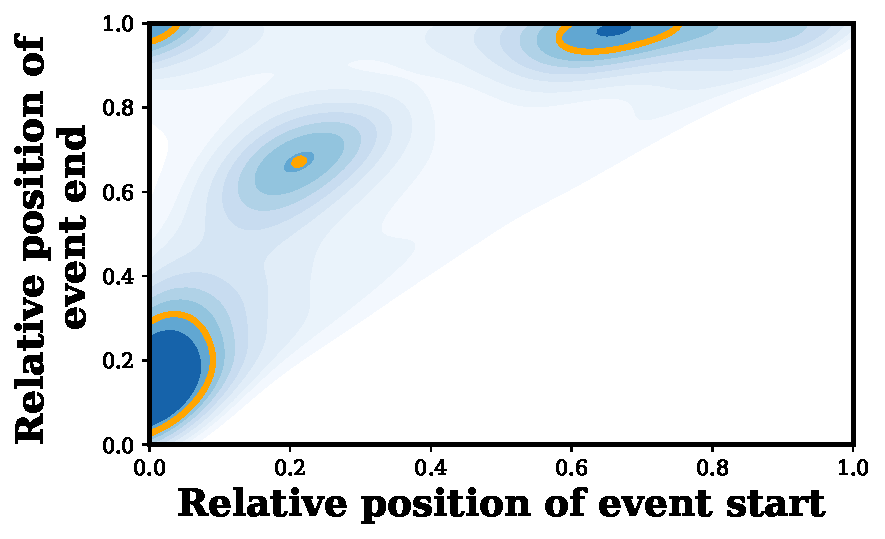
\includegraphics[width=\linewidth]{img/bias_anet.pdf}
        \caption*{(a)
        }
    \end{minipage}
    \hfill
    \begin{minipage}[t]{0.32\linewidth}
        \centering
        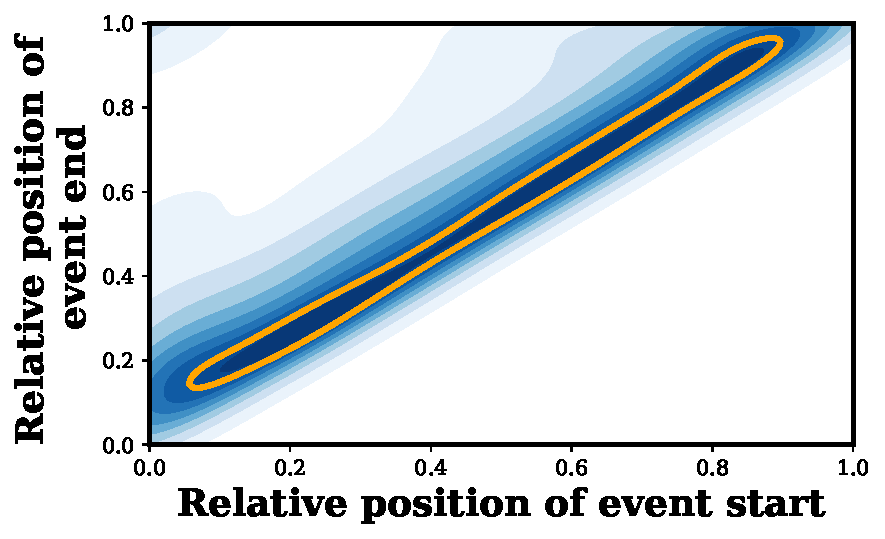
\includegraphics[width=\linewidth]{img/bias_qvhl.pdf}
        \caption*{(b)
        }
    \end{minipage}
    \hfill
    \begin{minipage}[t]{0.32\linewidth}
        \centering
        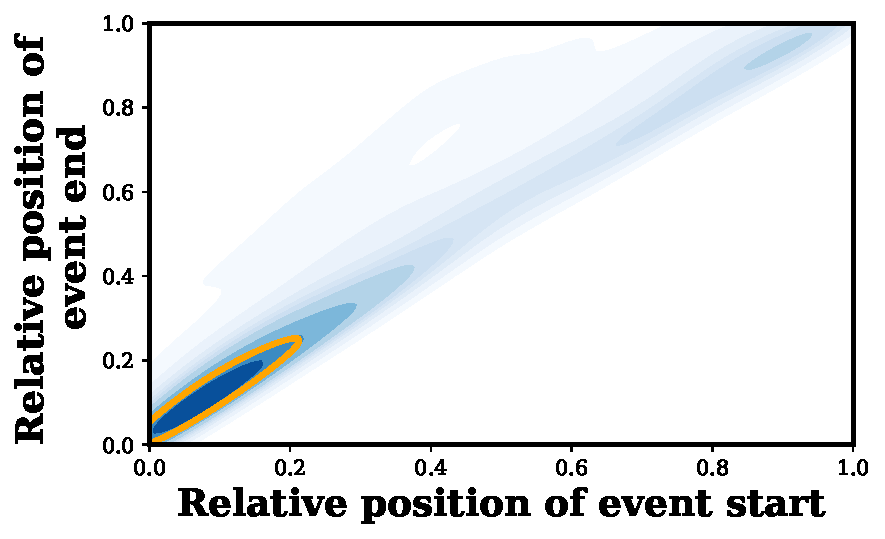
\includegraphics[width=\linewidth]{img/bias_tacos.pdf}
        \caption*{(c)
        }
    \end{minipage}
    \caption{Temporal distribution bias in
        (a) ANet-Captions.  
        (b) QVHighlights.  
        (c) TACoS.
        \textcolor{navy}{Darker colors} indicate higher data density.
        , and the \textcolor{yellow}{yellow curve} outlines the region of greatest density.
    }
\label{fig:bias_all}
\end{figure}

\subsubsection{Decomposition of Query}
The prompts provided to \texttt{Qwen2}~\cite{qwen2} for decomposing each Charades-STA query into a set of object-centric questions are as follows:

\begin{lstlisting}
System:
You are Qwen, created by Alibaba Cloud. You are a helpful assistant.
System:
Analyze the given query and:
1. Identify ONLY concrete, specific objects (nouns) that are:
   - Tangible physical items
   - Clearly named (not pronouns/ambiguous)
2. STRICTLY EXCLUDE:
   - All human references (person, he, she, they, etc.)
   - Ambiguous terms (something, anything, things, etc.)
   - Pronouns (it, they, them)
   - Abstract concepts
3. For each valid object, generate EXACTLY ONE question:
   "When does [OBJECT] appear?"

Negative Examples (BAD):
Input: "Someone left some items on the furniture"
Wrong Output:
-When does the furniture appear?
-When does some items appear?  # <-- AMBIGUOUS TERM SHOULD BE EXCLUDED

Positive Examples (GOOD):
Input: "The machine processed the raw materials during the night"
Output:
-When does the machine appear?
-When does the raw materials appear?
-When does the night appear?
User:
Analyze: @<query>@
\end{lstlisting}

\subsection{Downstream Task Details}
\label{sub:donwstream}
\subsubsection{VideoQA with Temporal Grounding}

We use \texttt{Qwen2-VL-7B} as the VideoQA model for answer generation. By default, it processes long videos by uniformly sampling 32 frames. However, this sampling strategy may lead to the omission of critical information. To investigate whether temporal grounding models can compensate for this issue, we adopt the following procedure. First, we use different video temporal grounding models to localize the relevant segments for each question. Then, we crop the localized video intervals and input them into \texttt{Qwen2-VL-7B}. Specifically, for cropped video segments shorter than 32 seconds, we extend their duration from the center to 32 seconds. Within each interval, we again uniformly sample 32 frames for answer generation.

\subsubsection{Prompt template for VideoQA}
We use the same prompt template for all multiple-choice VideoQA benchmarks:

\begin{lstlisting}
System:
You are a helpful assistant.
User: 
@<video>@
Question: @<question>@
Options:
(A) @<Option_A>@
(B) @<Option_B>@
(C) @<Option_C>@
(D) @<Option_D>@
Please only give the best option.
Best Option:
Assistant:
\end{lstlisting}

\section{Additional Implementation Details}
\label{sec:implementation}

\subsection{Prompt template for UniTime}
\label{sub:prompt_unitime}

The prompt template used for coarse-grained segment retrieval as follows:

\begin{lstlisting}
System:
You are a helpful assistant.
User: 
@<timestamps & frames>@
This is a sequence interleaved with timestamps and frames. 
Your task is to identify the specific timestamp(s) when the given query appears.
Query: @<Query>@
Answer:
Assistant:
\end{lstlisting}

The prompt template used for fine-grained temporal grounding as follows:

\begin{lstlisting}
System:
You are a helpful assistant.
User: 
@<timestamps & frames>@
This is a sequence interleaved with timestamps and frames. 
Your task is to identify the temporal window (start and end timestamps) when the given query appears.
Query: @<Query>@
Answer:
Assistant:
\end{lstlisting}

\subsection{Video-centric Training}
\label{sub:vc}
\begin{wrapfigure}{r}{0.4\linewidth}
\vspace{-15pt}
    \centering
    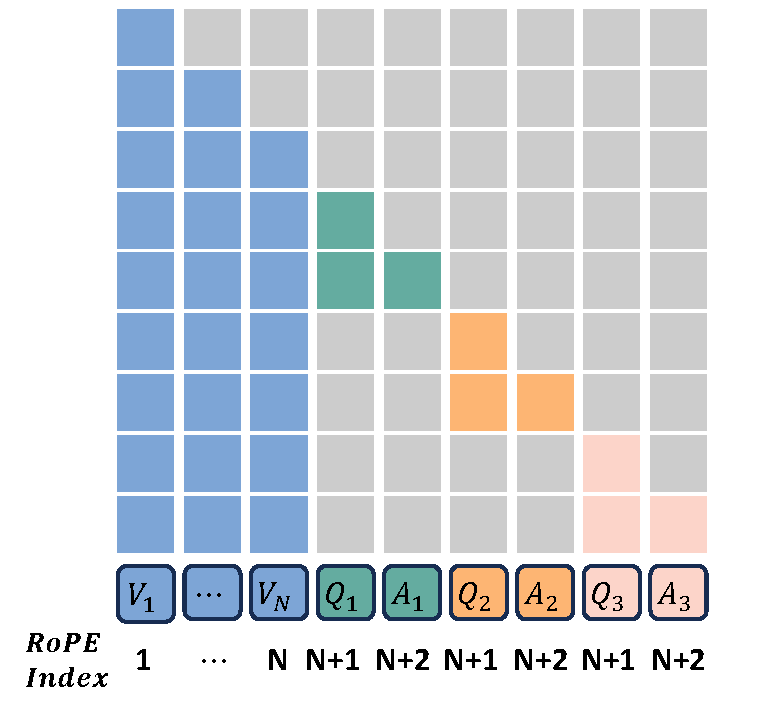
\includegraphics[width=0.9\linewidth]{img/vc3.pdf}
    \caption{
        Illustration of the video-centric training paradigm.
    }
    \label{fig:vc}
\end{wrapfigure}

In video-centric training, we first sample a video from the dataset and gather all associated queries with their corresponding answers. These queries and answers are concatenated and paired with the video as input, 
forming a sequence such as
\[
\begin{bmatrix}
v_1,\, v_2,\, \ldots,\, v_N,\, Q_1,\, A_1,\, Q_2,\, A_2,\, \ldots,
Q_{N_\text{sample}},\, A_{N_\text{sample}}
\end{bmatrix}
\].
As illustrated in Figure~\ref{fig:vc}, we apply attention masks to 
prevent different queries and answers from attending to others. Additionally, each query-answer sequence is assigned the same starting Rotary Position Embedding index, immediately following the indices of the video tokens.

\section{Qualitative Results}
\label{sec:qualitative}

\subsection{Qualitative Results for Ego4D-NLQ}
In Figure~\ref{fig:qualitative}, we present qualitative results of UniTime on Ego4D-NLQ. In the success cases, UniTime demonstrates precise coarse-grained segment retrieval and fine-grained temporal grounding capabilities. Despite the limited variation in video scenes, which are primarily composed of fine-grained interactions between hands and objects, the model consistently demonstrates robust performance.
In the failure cases, although the model retrieves the correct segment, it fails in fine-grained localization. As shown in the specific localization frames, this error occurs because the object referred to in the query appears multiple times in the video, while the ground truth only includes one of these occurrences.

\begin{figure}[htbp]
    \centering
    \begin{subfigure}{0.9\textwidth}
        \centering
        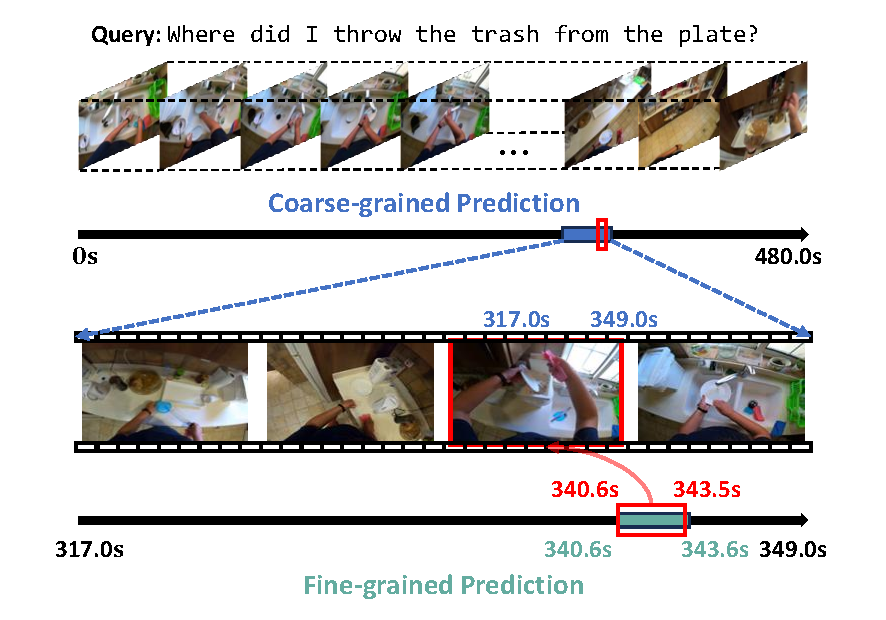
\includegraphics[width=\textwidth]{img/visualization1.pdf}
        \caption{success case}
    \end{subfigure}

    \vspace{1em}

    \begin{subfigure}{0.9\textwidth}
        \centering
        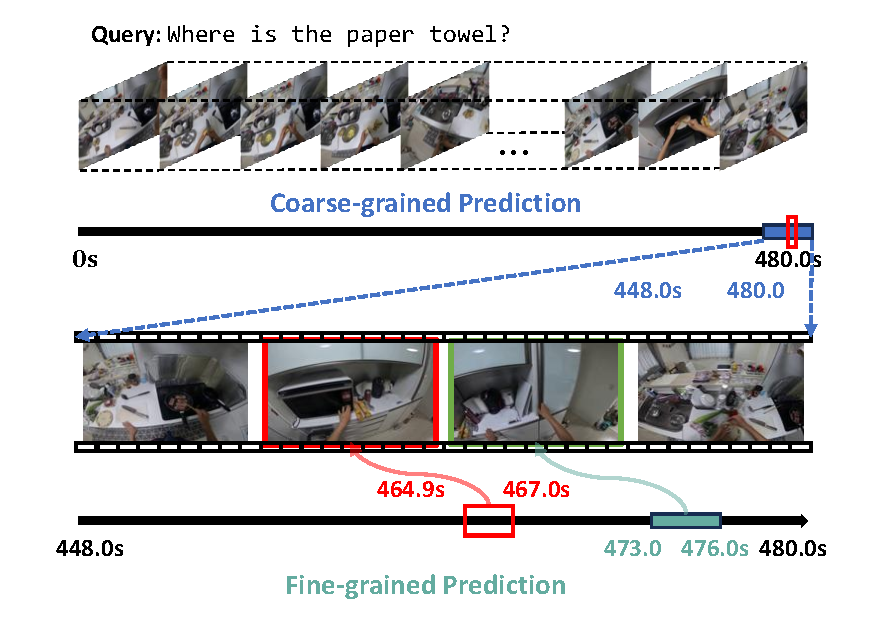
\includegraphics[width=\textwidth]{img/visualization2.pdf}
        \caption{failure case}
    \end{subfigure}

    \caption{Qualitative Results for long-video temporal grounding on the Ego4D-NLQ benchmark. \textcolor{figred}{\textbf{Red}} indicates the ground truth (GT), \textcolor{figblue}{\textbf{blue}} denotes the results of coarse-grained segment retrieval, and \textcolor{figgreen}{\textbf{green}} represents the results of fine-grained temporal grounding.}
    \label{fig:qualitative}
\end{figure}

\subsection{Qualitative Results for ANet-Captions}
\label{sub:anet}

As shown in Table 2, UniTime achieves substantial performance gains over competing methods across all benchmarks, except for ANet-Captions.
We analyze this discrepancy below, with Figure~\ref{fig:qualitative_short} visualizing UniTime’s predictions on ANet-Captions.

In successful cases (Figure~\ref{fig:qualitative_short}(a)), UniTime achieves precise temporal grounding. Despite the limited diversity of video scenes, which predominantly feature fine-grained interactions between hands and objects, the model consistently exhibits robust performance.

However, our analysis of the failure cases indicates that most can be traced to limitations in ANet-Captions's annotation scheme. As illustrated in Figure~\ref{fig:qualitative_short}(b), multiple occurrences of the same event are often annotated with only a single temporal interval. This occurs because captions are ordered sequentially, causing annotators to overlook recurring events.

Additionally, many failures arise from incorrect labels, as shown in Figure~\ref{fig:qualitative_short}(c).

\begin{figure}[htbp]
    \centering
    \begin{subfigure}{0.9\textwidth}
        \centering
        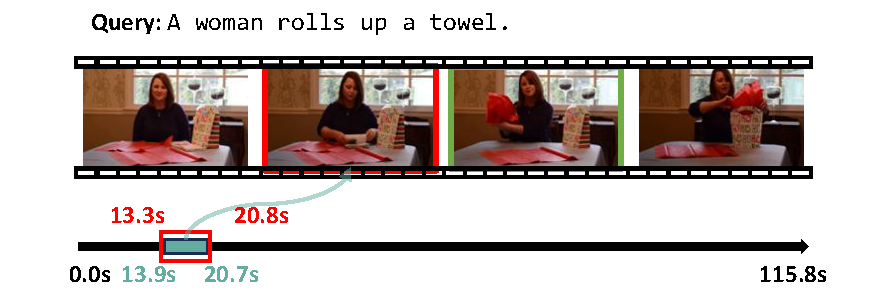
\includegraphics[width=\textwidth]{img/visualization_short1.pdf}
        \caption{Success case.}
    \end{subfigure}

    \vspace{1em}

    \begin{subfigure}{0.9\textwidth}
        \centering
        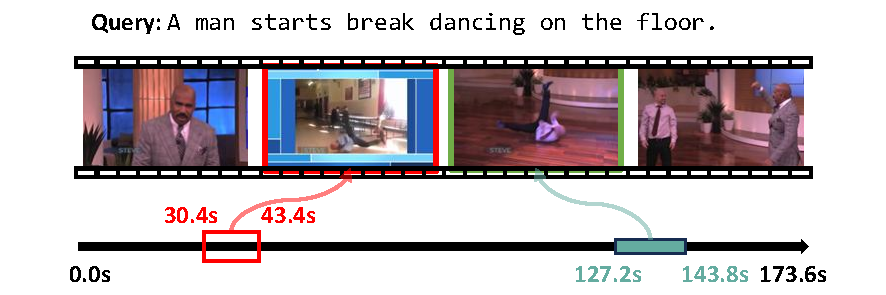
\includegraphics[width=\textwidth]{img/visualization_short3.pdf}
        \caption{Failure case resulting from incomplete annotations of multi-hop events.}
    \end{subfigure}

    \vspace{1em}

    \begin{subfigure}{0.9\textwidth}
        \centering
        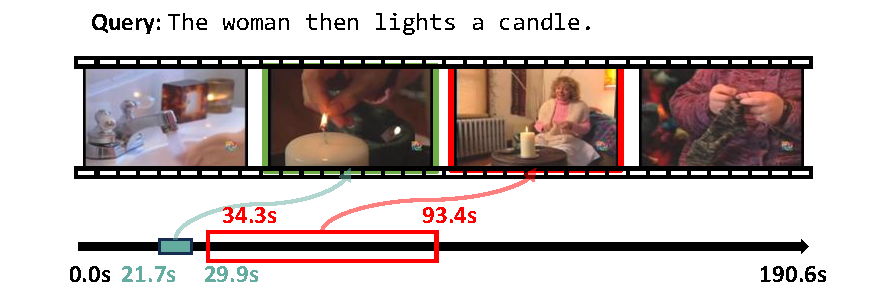
\includegraphics[width=\textwidth]{img/visualization_short2.pdf}
        \caption{Failure case caused by incorrect labels.}
    \end{subfigure}

    \caption{Qualitative Results for short-video temporal grounding on the ANet-Captions benchmark. \textcolor{red}{\textbf{Red}} indicates the ground truth (GT), \textcolor{figblue}{\textbf{blue}} denotes the results of coarse-grained segment retrieval, and \textcolor{figgreen}{\textbf{green}} represents the results of fine-grained temporal grounding.}
    \label{fig:qualitative_short}
\end{figure}

\section{Grounding Consistency Evaluation}
\label{sec:consistency}

To further evaluate UniTime’s robustness in temporal grounding, we conduct grounding consistency assessment on Charades-CON and ActivityNet-CON~\cite{jung2025consistency}, which are curated from subsets of CharadesSTA and ActivityNet-Captions, respectively. 
The grounding consistency targets two complementary consistency dimensions:

i) Rephrased Grounding (R-Ground). This metric evaluates whether a model’s moment predictions remain consistent across a query $q$ and its aligned rephrased variant $\hat{q}$. Concretely, the IoU between $m = \mathrm{Temp}_G(q)$ and $\hat{m} = \mathrm{Temp}_G(\hat{q})$ is computed. For each original query, the average IoU over three aligned variants is reported, reflecting the alignment consistency of predicted moments under paraphrasing.

ii) Shifted Grounding (S-Ground). This metric assesses whether a model consistently grounds the same visual content when that content is shifted to different temporal positions. Specifically, while preserving the internal frame sequence of the ground-truth moment $m_{\mathrm{gt}}$, it is randomly shifted to a new moment $m_s$, with evaluations conducted on the resulting predictions.

Experimental results, summarized in the Table~\ref{tab:ablation_consistency}, demonstrate that UniTime not only exhibits strong temporal grounding performance (Ground) but also achieves excellent consistency and robustness (R-Ground and S-Ground). UniTime attains performance comparable to VTune~\cite{jung2025consistency}, which extends instruction tuning with explicit consistency objectives, and in some cases surpasses it.

\begin{table}[t]
\caption{
\textbf{Grounding consistency evaluation of Video-MLLMs.} Relative consistency scores are in brackets.}
\vspace{3pt}
\centering
\resizebox{0.9\textwidth}{!}{
\setlength{\tabcolsep}{0.45cm}
\begin{tabular}{l * {6}{c}}  % 1 left-aligned + 12 centered columns
        \toprule
        \multirow{2}{*}{Method} & \multicolumn{3}{c}{\textbf{Charades-CON}} & \multicolumn{3}{c}{\textbf{ActivityNet-CON}} \\
        \cmidrule(lr){2-4} \cmidrule(lr){5-7} 
        & Ground & R-Ground & S-Ground & Ground & R-Ground & S-Ground \\
        \midrule
        GPT-4o~\cite{openai2024gpt4o} & 28.5 & 21.2 (74.3) & 9.3 (32.8) & 26.8 & 18.1 (67.5) & 10.4 (38.8) \\
        Gemini 1.5 Flash~\cite{team2024gemini} & 34.6 & 29.7 (85.7) & 24.8 (71.7) & 37.8 & \textbf{30.8 (81.4)} & \textbf{24.8 (65.6)} \\
        Video-LLaMA~\cite{zhang2023video} & 14.2 & 10.6 (74.9) & 5.3 (37.6) & 12.8 & 8.5 (66.8) & 7.2 (56.8) \\
        Video-LLaMA + VTune~\cite{jung2025consistency} & 54.4 & 38.2 (70.3) & 10.9 (20.0) & 33.0 & 24.7 (74.8) & 10.0 (30.2) \\
        TimeChat~\cite{ren2024timechat} & 30.5 & 25.0 (82.1) & 5.6 (18.5) & 4.6 & 2.9 (64.1) & 1.0 (21.2) \\
        TimeChat + VTune~\cite{jung2025consistency} & 76.2 & 69.2 \textbf{(90.8)} & 36.2 (47.5) & 37.4 & 28.3 (75.6) &  10.6 (28.3) \\
        UniTime-Full & \textbf{81.5} & \textbf{73.9} (90.7) & \textbf{58.3 (71.6)} & \textbf{49.1} & 30.2 (61.5) & 21.3 (43.4) \\
        \bottomrule
        \end{tabular}}
\label{tab:ablation_consistency}
\end{table}

\section{More Ablation Studies}
\label{sec:ablation}

\subsection{Effect of Video Processing Strategies}
\label{sub:input_process}
To justify our design choice in Section~\ref{sec:architecture}, i.e., resizing short videos and compressing long videos, we conduct an ablation study on the Ego4D-NLQ dataset. This study evaluates how different video processing strategies impact both grounding performance and computational efficiency.

\begin{table}[h]
\caption{
\textbf{Ablation on video processing strategies.} Seg Retrieval Acc. indicates the accuracy of coarse-grained segment retireval.}
\vspace{3pt}
\centering
\resizebox{\textwidth}{!}{
\setlength{\tabcolsep}{0.45cm}
\begin{tabular}{*{7}{c}}  % 1 left-aligned + 12 centered columns
        \toprule
        Short Video & Long Video & R1@.3 & R1@.5 & mIoU & Seg Retrieval Acc. & Training Time \\
        \midrule
        Frame Resizing & Token Compression & 24.79 & 16.83 & 17.25 & 45.28 & 21 h \\
        Frame Resizing & Frame Resizing & 18.53 & 12.67 & 12.88 & 35.36 & 12 h \\
        Token Compression & Token Compression & 24.06 & 16.18 & 16.71 & 45.28 & 24.5 h \\
        \bottomrule
        \end{tabular}}
\label{tab:ablation_process}
\end{table}

Our findings indicate that: (i) For long videos, adaptive frame scaling reduces tokens per frame while keeping the frame rate fixed. Though some visual cues are lost, this feature-level token compression retains more semantic information than frame resizing, which discards input resolution. This leads to better segment retrieval accuracy and recall (row 1 vs. row 2). (ii) For short clips with sufficient tokens, both methods perform similarly (row 1 vs. row 3). However, token compression requires high-resolution inputs before merging, incurring higher computational costs. In UniTime-Full, using token compression for short videos increased training time by 5 days compared to frame resizing. 

Therefore, rather than employing a unified strategy, we adopt a hybrid approach to balance performance and efficiency: for short videos, we apply frame resizing to reduce computational overhead, while for long videos, we leverage token compression to better preserve visual details. This design choice enables our method to achieve strong performance with practical training costs.

\subsection{Comparison of Temporal Information Encoding}
\label{sub:temporal encoding}

We conduct ablation experiments on Charades-STA to compare the effectiveness of Timestamp Token Insertion versus Dense Position Encodings.

\begin{table}[h]
\caption{
\textbf{Ablation on temporal information encoding.}}
\vspace{3pt}
\centering
\resizebox{.9\textwidth}{!}{
\setlength{\tabcolsep}{0.45cm}
\begin{tabular}{l * {3}{c}}  % 1 left-aligned + 12 centered columns
        \toprule
        Method & R1@.5 & R1@.7 & mIoU \\
        \midrule
        Dense Position Encodings & 48.44 & 27.15 & 44.85 \\
        Timestamp Token Insertion (UniTime-SP) & 74.33 & 53.71 & 63.15 \\
        \bottomrule
        \end{tabular}}
\label{tab:ablation_encoding}
\end{table}

Our base model, \texttt{Qwen2-VL-7B}, utilizes Multimodal Rotary Position Embedding (MRoPE), which decomposes position embeddings into temporal, height, and width components. After fine-tuning, temporal grounding remains suboptimal with dense position encodings.
In contrast, timestamp token insertion yields significant gains. We attribute this improvement to the MLLM's strong multimodal retrieval ability and the simplification of the task into (i) identifying question-relevant video segments and (ii) directly reading their corresponding timestamp tokens.

\subsection{Ablation Study of Adaptive Frame Scaling Hyperparameters}
\label{sub:hyper}

In this section, we conduct an ablation study on the threshold hyperparameters $N_f^{\text{long}}$, $N_f^{\text{short}}$, and the token budget $N_{\text{total}}$ within Adaptive Frame Scaling, elucidating the rationale behind our parameter choices.

\noindent \textbf{Threshold $N_f^{long}$.} This parameter specifies the maximum video length that can be processed in a single pass.
For videos with length $\leq N_f^{\text{long}}$, we process the input directly; for videos with length $> N_f^{\text{long}}$, we partition the input into segments, process each segment independently, and then aggregate the predictions. As shown in Table~\ref{table:abl_nflong}, varying $N_f^{\text{long}}$ has only a marginal effect on accuracy because over-length inputs are segmented and subsequently fused. Moreover, Adaptive Frame Scaling maintains a fixed token budget per segment, so reducing $N_f^{\text{long}}$ increases the number of segments and the total token count at inference, thereby incurring higher latency. Balancing efficiency and accuracy, we set $N_f^{\text{long}}=1024$.

\noindent \textbf{Threshold $N_f^{short}$.} This hyperparameter determines whether inference is executed in a single stage or via a multi-stage (coarse-to-fine) pipeline. For inputs with temporal length $\leq N_f^{\text{short}}$, we use single-stage processing; for inputs with temporal length $> N_f^{\text{short}}$, we employ multi-stage processing. As shown in Table~\ref{table:abl_nfshort}, within the 64–128 s duration range, the performance difference between multi-stage ($N_f^{\text{short}}{=}64$) and single-stage ($N_f^{\text{short}}\geq 128$) configurations is modest. However, a lower threshold increases average inference latency by routing more inputs to the multi-stage pipeline. For inputs in the 128–256 s range, multi-stage processing yields substantially higher accuracy (54.57 vs. 42.90 mIoU). To balance accuracy and efficiency, we set $N_f^{\text{short}}{=}128$.

\noindent \textbf{Token budget $N_{\text{total}}$.} This parameter specifies the maximum number of tokens permitted. As shown in Table~\ref{table:abl_total}, performance improves monotonically as the token budget increases, up to the available GPU capacity. Accordingly, we set $N_{\text{total}}=16,384$, which corresponds to the upper limit supported by our hardware.

\begin{table}[t]
\begin{minipage}[t]{0.3\textwidth}
    \centering
    \captionof{table}{
    \textbf{Ablation of the threshold $N_f^{\text{long}}$ on Ego4D.}}
    \label{table:abl_nflong}
    \resizebox{\textwidth}{!}{
    \setlength{\tabcolsep}{0.15cm}
    \begin{tabular}{*{4}{c}}
    \toprule
    $N_f^{long}$ & R1@.3 & R1@.5 & mIoU \\
    \midrule
    1024 & 24.79 & 16.83 & 17.25 \\
    512 & 24.72 & 16.63 & 16.95 \\
    256 & 23.94 & 16.10 & 16.68 \\
    \bottomrule
    \end{tabular}}
\end{minipage}%
\hfill
\begin{minipage}[t]{0.32\textwidth}
    \centering
    \captionof{table}{
    \textbf{Ablation of the threshold $N_f^{\text{short}}$ on TaCoS.}}
    \label{table:abl_nfshort}
    \resizebox{\linewidth}{!}{
    \setlength{\tabcolsep}{0.15cm}
    \begin{tabular}{*{4}{c}}
    \toprule
    \multirow{2}{*}{$N_f^{short}$} & mIoU & mIoU & mIoU \\
    & (64-128s) & (128-256s) & Avg. \\
    \midrule
    64 & 58.43 & 54.57 & 50.28 \\
    128 & 56.59 & 54.57 & 50.00 \\
    256 & 56.59 & 42.90 & 46.82 \\
    \bottomrule
    \end{tabular}}
\end{minipage}
\hfill
\begin{minipage}[t]{0.3\textwidth}
    \centering
    \captionof{table}{
    \textbf{Ablation of the token budget $N_{\text{total}}$ on Ego4D.}}
    \vspace{2pt}
    \label{table:abl_total}
    \resizebox{\linewidth}{!}{
    \setlength{\tabcolsep}{0.15cm}
    \begin{tabular}{*{4}{c}}
    \toprule
    Budget & R1@.3 & R1@.5 & mIoU \\
    \midrule
    16384 & 24.79 & 16.83 & 17.25 \\
    8192 & 24.08 & 16.10 & 16.69 \\
    4096 & 23.04 & 15.07 & 15.96 \\
    \bottomrule
    \end{tabular}}
\end{minipage}
\end{table}

% \subsection{Effect of Model Size.}
% \label{sub:size}

% To assess the impact of MLLM capacity, we ablate model size on Ego4D-NLQ and Charades-STA. As Table~\ref{tab:ablation_model_size} shows, the larger \texttt{Qwen2-VL-7B} outperforms its smaller counterpart \texttt{Qwen2-VL-2B}.
% This suggests that increased model capacity enhances multimodal reasoning, thereby further improving temporal grounding performance when integrated with our proposed method.

% \begin{table}[h]
% \caption{
% \textbf{Ablation on model size.}
% All experiments are conducted under the dataset-specific setting.}
% \vspace{3pt}
% \centering
% \resizebox{.9\textwidth}{!}{
% \setlength{\tabcolsep}{0.45cm}
% \begin{tabular}{l *{7}{r}}  % 1 left-aligned + 12 centered columns
%         \toprule
%         \multirow{2}{*}{MLLMs} &  \multirow{2}{*}{Size} &
%         \multicolumn{3}{c}{\textbf{Charades-STA}} & 
%         \multicolumn{3}{c}{\textbf{Ego4D-NLQ}}  \\
%         \cmidrule(lr){3-5} \cmidrule(lr){6-8}
%          & & R1@.5 & R1@.7 & mIoU & R1@.3 & R1@.5 & mIoU \\
%         \midrule
%         Qwen2-VL & 2B & 65.38 & 42.18 & 57.25 & 10.50 & 5.80 & 7.29 \\
%         Qwen2-VL & 7B & \textbf{74.33} & \textbf{53.71} & \textbf{63.15} & \textbf{24.79} & \textbf{16.83} & \textbf{17.25}\\
%         \bottomrule
%         \end{tabular}}
% \label{tab:ablation_model_size}
% \end{table}

% \subsection{Effect of Model Type.}
% \label{sub:type}
% As discussed in Section~2.2, our approach is compatible with any MLLM that can process dynamic frame inputs. To assess architectural impact, we evaluate two MLLM variants: \texttt{Qwen2-VL-7B} and \texttt{Qwen2.5-VL-7B}. As shown in Table~\ref{tab:ablation_model_type}, our method consistently achieves superior temporal grounding performance regardless of the underlying MLLM. These results demonstrate that the effectiveness of our framework can continually benefit from advances in MLLM architectures, enabling further improvements in temporal grounding as more powerful MLLMs become available.

% \begin{table}[h]
% \caption{
% \textbf{Ablation on model type.}
% All experiments are conducted under the dataset-specific setting.}
% \vspace{3pt}
% \centering
% \resizebox{\textwidth}{!}{
% % \setlength{\tabcolsep}{0.45cm}
% \begin{tabular}{l *{10}{r}}  % 1 left-aligned + 12 centered columns
%         \toprule
%         \multirow{2}{*}{MLLMs}  &
%         \multicolumn{2}{c}{\textbf{Charades-STA}} & 
%         \multicolumn{2}{c}{\textbf{ANet-Captions}} &
%         \multicolumn{2}{c}{\textbf{QVHighlights}} &
%         \multicolumn{2}{c}{\textbf{Ego4D-NLQ}} &
%         \multicolumn{2}{c}{\textbf{TaCoS}} \\
%         \cmidrule(lr){2-3} \cmidrule(lr){4-5} \cmidrule(lr){6-7} \cmidrule(lr){8-9} \cmidrule(lr){10-11}
%          & R1@.5 & R1@.7 & R1@.5 & R1@.7 & R1@.5 & R1@.7 & R1@.3 & R1@.5 & R1@.3 & R1@.5 \\
%         \midrule
%         Qwen2-VL-7B  & \textbf{74.33} & 53.71 & 54.81 & 36.62 & \textbf{77.76} & \textbf{63.29} & \textbf{24.79} & \textbf{16.83} & 61.18 & 48.31  \\
%         Qwen2.5-VL-7B & 74.19 & \textbf{53.98} & \textbf{55.64} & \textbf{37.64} & 77.17 & 63.10 & 23.53 & 16.12 & \textbf{61.61} & \textbf{49.16} \\
%         \bottomrule
%         \end{tabular}}
% \label{tab:ablation_model_type}
% \end{table}

\section{Limitations \& Future Work}
\label{sec:limitations}

While UniTime demonstrates exceptional performance on various video temporal grounding and video QA benchmarks, it still has several limitations that warrant further exploration:
(i) UniTime is currently constrained to temporal grounding tasks. To enable broader applications in MLLMs, it requires more diverse training data with dense temporal annotations. Incorporating such data into the pretraining process of MLLMs could unlock their potential for handling more temporally complex tasks, such as dense video captioning.
(ii) Although UniTime enhances MLLMs with temporal grounding capabilities, relying solely on temporal grounding data limits their reasoning and question-answering abilities. The ultimate objective is to develop MLLMs that seamlessly integrate localization, reasoning, and question-answering into a unified framework.
(iii) The current approach to processing long videos in UniTime relies on a fixed segment length, which lacks flexibility. Future work could investigate adaptive segment lengths based on the information density of videos, enabling more efficient and context-aware video processing.

\section{Broader Impacts Statement}
\label{sec:impacts}

Our research advances the field of video understanding by developing more accurate and efficient models for temporal grounding and video question answering. While temporal grounding with UniTime offers significant benefits for a variety of video understanding applications, unexpected behaviors may occasionally result in misrepresentations of the underlying video content. For applications that demand extremely precise temporal localization for safety-critical decisions, such as embodied intelligence tasks, it is crucial to carefully manage any such behaviors. To ensure the reliability of systems that rely on temporal grounding predictions, we recommend conducting thorough evaluations and implementing robust mitigation strategies to minimize potential risks. Through these precautions, the overall safety and effectiveness of these applications can be substantially enhanced.
